\begin{frame}{Abstract}
	In this Master's Thesis, I study the effects of the backreaction of a charged Klein-Gordon field coupled to an external classical electric field, in 1+1 dimensional spacetime.

	The calculations are done w.r.t. Hadamard point-split renormalization, which presents relevant corrections to previous work for this problem. 

In this Research Practice, I state and motivate the problem I intend to solve, and compare the renormalization technique I will be using with the one that has already been used. 
\end{frame}

\section{Introduction}

\begin{frame}{Motivation}
	\begin{itemize}[<+->]
	\item \textbf{Historically} Vacuum polarization was one of the first quantum electrodynamical effects theoretically studied. Introduces non-linear term in Maxwell equations.
	\item \textbf{In practice} it provides corrections to atomic energy levels  [Mohr 1998 qed corrections in heavy atoms] 
	\item \textbf{Interest has revived} in the context of topological insulators [Fialkovsky 2019 Quantum Dirac fermions in a halp space\ldots]
	\item  \textbf{These calculations }were already done [ambjorn wolfam 1983], but present counter intuitive results, such as anti-screening behavior for Neumann boundary conditions.
		\begin{enumerate}
			\item Vacuum polarization calculations through mode sum formula
			\item Not considering relevant solutions for the Neumann boundary conditions.
		\end{enumerate}
\end{itemize}
	
\end{frame}

\begin{frame}{The problem}
	\begin{center}
	\begin{tikzpicture}[
	    node distance=2cm,
	    main/.style = {draw, circle, minimum size=1.2cm, thick},
	    rect/.style = {draw, rectangle, minimum width=2.5cm, minimum height=1cm, thick},
	    every edge/.append style={-{Latex[scale=1.2]}, thick}
	]
	
	% Nodes
	\node[main] (KG) {$\phi$};
	\node[rect, right=2.7cm of KG] (Charge) {$\rho$};
	\node[rect, below=2.7cm of Charge] (Field) {$\vec{E}$};
	
	% Edges
	\draw[->] (KG) -- (Charge) node[midway, above] {Contributes to};
	\draw[->] (Charge) -- (Field) node[midway, right] {Interacts with};
	\draw[->] (Field) -- (KG) node[midway, left] {Influences};
	
	% Back reaction loop
	\path[->] (Field) edge [bend left=45] (KG);
	
	% Labels
	%\node[above] at (current bounding box.north) {Back Reaction with a Klein-Gordon Field in an External Electric Field};
	
	\end{tikzpicture}
	
\end{center}

\end{frame}

\section{Methods}
\begin{frame}{The set up}
	\begin{themedTitleBlock}{Klein-Gordon equation}
	We study a $1+1$ dimensional Klein-Gordon field coupled to a external classical electromagnetic vector potential $A_\mu(x)$
	\begin{align}
		(D_\mu D^\mu + m^2) \phi = 0,
	\end{align}
	with
	\begin{enumerate}
		\item $D_\mu = \partial_\mu + i e A_\mu$ the covariant derivative
		\item $(+, -)$ the metric signature
		\item $x^\mu = (x^{0}, x^{1}) \in \mathbb{R} \times [0, a]$
	\end{enumerate}
	\end{themedTitleBlock}
\end{frame}

\begin{frame}{Boundary conditions}
	We restrict the field to the interval $x^{1}\in [0, a]$
	\uncover<1->{
		\begin{themedTitleBlock}{Robin Boundary Conditions}
			\vspace{-0.3cm}
			\begin{align}
				\frac{\partial \phi(0)}{\partial x^{1}} = h_0\phi (0),  \hspace{1.5cm}
				\frac{\partial \phi(a)}{\partial x^1} = -h_a\phi (a), 
			\end{align}
		\end{themedTitleBlock}
	}
	\begin{enumerate}
		
	\uncover<2->{
		\item
			\alert{Dirichlet} If we let $h_i \to \infty$ 
			\begin{align}
				\phi(0) = \phi(a) = 0, 
			\end{align}
	}
	\uncover<3->{
		\item
			\alert{Neumann} If we let $h_i \to 0$,
			\begin{align}
				\frac{\partial \phi(0)}{\partial x^{1}} = 
				\frac{\partial \phi(a)}{\partial x^{1}} = 0
			\end{align}
	}
	\end{enumerate}

\end{frame}

\begin{frame}{Electromagnetic potential}
	\begin{columns}
	    \begin{column}{0.5\textwidth}
\begin{figure}[ht]
    \centering
    \incfig{the-background-classical-electric-field}
    \caption{The background classical electric field}
    \label{fig:the-background-classical-electric-field}
\end{figure}
	    \end{column}
	    \begin{column}{0.5\textwidth}
		    \begin{enumerate}[<+->]
		    	\item 
	    Constant electric field of strength $E$ pointing towards positive $x^{1}.$
    \item Under the Coulomb gauge $$A_0(x^{1}) = -Ex^{1},\, A_1(x_0) = 0$$ up to additive constant
    \item To ensure anti-symmetric solutions $$A_0(x^{1})=-E(x^{1}-\frac{a}{2})$$

		    \end{enumerate}
	    \end{column}
	\end{columns}

\end{frame}
\begin{frame}{Electromagnetic potential}
	\begin{columns}
	    \begin{column}{0.5\textwidth}
\begin{figure}[ht]
    \centering
    \incfig{the-background-classical-electric-field-and-potential}
    \caption{The background classical electric field and potential}
    \label{fig:the-background-classical-electric-field-and-potential}
\end{figure}
	    \end{column}
	    \begin{column}{0.5\textwidth}
		    \begin{enumerate}
		    	\item 
	    Constant electric field of strength $E$ pointing towards positive $x^{1}.$
    \item Under the Coulomb gauge $$A_0(x^{1}) = -Ex^{1},\, A_1(x_0) = 0$$ up to additive constant
    \item To ensure anti-symmetric solutions $$A_0(x^{1})=-E(x^{1}-\frac{a}{2})$$

		    \end{enumerate}
	    \end{column}
	\end{columns}
\end{frame}

\begin{frame}{Time independent Klein-Gordon equation}
	\uncover<1->{
These considerations and the variable separation ansatz $\phi(x) = \phi_n(x^{1})e^{-i\Omega_n x^{0}}$ yield 
	}
	
	\uncover<2->{
	\begin{themedTitleBlock}{Mode equation}
		\vspace{-0.3cm}
		\begin{align}
			\left( \left[ \Omega_n - eA_0(x^{1})  \right]^2 + \frac{d^2}{d \left( x^1 \right) ^2} + m^2  \right) \phi_n &= 0 \\
			\left( \left[ \Omega_n + eE \left(  x^{1} - \frac{a}{2}\right)  \right]^2 + \frac{d^2}{d \left( x^1 \right) ^2}  + m^2\right) \phi_n &= 0
		\end{align}
	\end{themedTitleBlock}
	}
\end{frame}

\begin{frame}{Dimensionless parameters}
	We introduce the dimensionless coordinates
		\begin{align}
			\left( x^{0}, x^{1} \right) \to (t, z) :=\left(  \frac{x^{0}}{a},\frac{x^{1}}{a}\right)  \in \R \times [0, 1],
		\end{align}
	and define $$\phi(t, z) := \phi\left( \frac{x}{a} \right) ,\,\, A_0(z) := -Ea\left( z-\frac{1}{2} \right)$$
	This way, the mode equation can be written as 
		\begin{align}
			\left( \left[ a\Omega_n - eaA_0(z)  \right]^2 + \frac{d^2}{dz^2} + a^2m^2  \right) \phi_n &= 0 \\
			\left( \left[ a\Omega_n + ea^2E \left( z-\frac{1}{2} \right)   \right]^2 + \frac{d^2}{dz^2} + a^2m^2  \right) \phi_n &= 0
		\end{align}
\end{frame}

\begin{frame}{Dimensionless parameters}
	\uncover<1->{
		Lastly, introduce the dimensionless parameters
	\begin{enumerate}
		\item  $\lambda = ea^2E$
	
		\item  $\epsilon = ea$
		\item $\omega_n = a\Omega_n$
	\end{enumerate}
	}
	
	\uncover<2->{
\begin{themedTitleBlock}{Dimensionless Klein-Gordon equation}
	\vspace{-0.3cm}
		\begin{align}
			\left( \left[ \omega_n - \epsilon A_0(z)  \right]^2 + \frac{d^2}{dz^2} + a^2m^2  \right) \phi_n &= 0 \\
			\left( \left[ \omega_n + \lambda \left( z-\frac{1}{2} \right)   \right]^2 + \frac{d^2}{dz^2} + a^2m^2  \right) \phi_n &= 0
		\end{align}
\end{themedTitleBlock}
	}
\end{frame}

\begin{frame}{The external field approximation}
	Without taking backreaction into account, the KG equation can be solved by
\begin{align*}
	\phi_n(z) &= 
	a_n D_{i \frac{a^2m^2}{2\lambda} - \frac{1}{2}} \left( 
		\frac{1+i}{\sqrt{\lambda} }
		\left( \omega_n + \lambda \left( z-\frac{1}{2} \right)
		\right) 
	\right) 
	\\
		  &+
	b_n D_{-i \frac{a^2m^2}{2\lambda} - \frac{1}{2}} \left( 
		\frac{i - 1}{\sqrt{\lambda} }
		\left( \omega_n + \lambda \left( z-\frac{1}{2} \right)
		\right) 
	\right)
	\label{eq:parabolyc-cylinder}
\end{align*}
with $D_\nu(z)$ the parabolic cylinder functions.
\end{frame}

\begin{frame}{The external field approximation -- Perturbation theory}
\uncover<1->{
	We want to turn the problem in to a Schrödinger-like equation
	\begin{align}
		i\partial_t \ket{\Psi} = H\ket{\Psi}, 
		\text{with} \ket{\Psi} = \begin{pmatrix} \phi \\ \pi^* \end{pmatrix}, \,\text{and}\, \pi^* = D_0\phi
	\end{align}
}

\uncover<2->{
	The corresponding Hamiltonian would be 
	\begin{align}
		H = \underbrace{i \begin{pmatrix} 0 & 1 \\
		D_1^2 -m^2 & 0 
	\end{pmatrix}}_{H_0}+
	\underbrace{			\begin{pmatrix} eA_0 & 0 \\
				0 & eA_0
		\end{pmatrix}}_{H_1}.
	\end{align}
}
\uncover<3->{
Which is hermitian w.r.t. 
\begin{align}
	\bra{\Psi_1}\ket{\Psi_2} = i \int_{0}^{1} dz \left( \phi_1^{*}\pi_2^* -  \pi_{1} \phi_2 \right)  
\end{align}
}
\end{frame}

\begin{frame}{The external field approximation -- Perturbation theory}
	\uncover<1->{
	\begin{align}
		\omega_n ^{(1)} &= \frac{\bra{\Psi_n^{(0)}}\ket{H_1\Psi_n^{(0)}}}{\bra{\Psi_n^{(0)}}\ket{\Psi_n^{(0)}}} \\
		\ket{\Psi_n ^{(1)}} &= \sum_{k\neq n}^{} 
		\frac{
			1
		}
		{
		\bra{\Psi_n^{(0)}}\ket{\Psi_n^{(0)}}
		}
		\frac{
		\bra{\Psi_k^{(0)}}\ket{H_1\Psi_n^{(0)}}
		}{
		\omega_n ^{0} - \omega_k^{(0)}
		} \ket{\Psi_k^{(0)}}
	\end{align}
	}
	
	\uncover<2->{
	One finds that perturbation theory yields \textbf{no correction} to the eigenvalues $$\omega_n^{D, N} = \text{sgn}(n) \sqrt{a^2m^2 + \pi^2n^2}.$$ 
	}

\end{frame}
\begin{frame}{The external field approximation -- Perturbation theory}
	\uncover<1->{
		For \alert{Dirichlet} boundary conditions
	\begin{align}
		\begin{split}
			\phi_n^{D} &= \left( m^2 + \pi^2  n^2 \right)^{-\frac{1}{2}} \left[ \sin\pi n z \right.\\
				   &\left.+ \lambda \frac{\sqrt{m^2 + \pi^2 n^2} }{2 \pi \lvert n \rvert} 
				\left( 
				\frac{1}{\pi n}\left( \frac{1}{2} - z \right) \sin \pi n z - z(1-z) \cos \pi n z \right) 
			\right] 
		\end{split}
	\end{align}
	}
	
	\uncover<2->{
		For \alert{Neumann} boundary conditions
		\begin{align}
			\begin{split}
				\phi_n^{N} &= \left( m^2 + \pi^2 n^2 \right)^{-\frac{1}{2}} 
				\left[ \cos\pi n z  \right. \\
					   &\left. + \lambda \frac{\sqrt{m^2 + \pi^2 n^2} }{2 \pi \lvert n \rvert} 
					\left( 
					\frac{1}{\pi n}\left( \frac{1}{2} - z \right) \cos \pi n z 
				+ ( z(1-z) + (\pi n)^{-2} ) \sin \pi n z \right) 
				\right] 
			\end{split}
		\end{align}
	}
	

\end{frame}

\begin{frame}{Quantization and renormalization}
We quantize the field based on the mode solutions 
\begin{align}
	\phi(t, z) = \sum_{n>0}^{} a_n \phi_n(z) e^{-i\omega_nt}
	+\sum_{n<0}^{} b_n^{\dagger} \phi_n(z) e^{-i\omega_nt},
\end{align}
with $a_n$, $b_n$ the operators fulfilling 
\begin{align}
	\left[ a_n, a_m^\dagger \right] = \delta_{nm}, \hspace{1cm}
	\left[ b_n, b_m^\dagger \right] = \delta_{nm}, \\
	\left[ a_n, a_m\right] =\left[ a_n, b_m\right] =\left[ a_n, b_m^\dagger\right] =\left[ b_n, b_m\right] = 0 .
\end{align}
This also defines the vacuum by
\begin{align}
	a_n \ket{0} = b_n \ket{0}  = 0	
\end{align}

\end{frame}

\begin{frame}{Charge density}
	\uncover<1->{
		We calculate the \textbf{charge density} as the 0th component of the charge current 
	\begin{align}
		\rho(z) = ie\bra{0} \phi^*(z) D_0 \phi(z) - \phi(z) D_0 \phi^*(z) \ket{0}
	\end{align}
	}
	
	\uncover<2->{
	Ambj\o rn and Wolfram calculate it as one naïvely would, 
	\begin{align}
		\rho(z) = e\left( \sum_{n>0}^{} (\omega_n - eA_0(z)) \lvert \phi_n(z)  \rvert ^2- \sum_{n<0}^{} (\omega_n - eA_0(z)) \lvert \phi_n(z) \rvert^2 \right) 
	\end{align}
	Which leads to incorrect results, such as non vanishing induced charges^* check this!
	}
\end{frame}

\begin{frame}{Hadamard states}

	\uncover<1->{
	Assume that the state is of Hadamard form,
	\begin{align}
		w^{\phi \phi^*}_\Omega(x, x') = \bra{\Omega}\phi(x) \phi^*(x')\ket{\Omega}  = H^{\phi \phi^*}(x, x')+ R_\Omega^{\phi \phi^*}(x, x'),
	\end{align}
}
\uncover<2->{
	with 
	\begin{align}
		H^{\phi \phi^*}(x, x') = -\frac{1}{4\pi} U(x, x') \log(-(x-x')^2 + i\epsilon (x-x')^{0})
	\end{align}
	and $$U(x,x') = \exp\left( -i \int_{0}^{1}A_\mu ( x' + s(x-x')) (x-x')^\mu ds   \right).$$
	}
	
	\uncover<3->{
	Define the product of derivatives of fields as 
	\begin{align}
		\bra{\Omega} D_\alpha\phi(x)(D_\beta\phi)^*(x)\ket{\Omega} =
		\lim_{x\to x'} \left[ D_\alpha D'_\beta^*\left( 
		w^{\phi \phi^*}_\Omega(x, x') - H^{\phi \phi^*}(x, x')
		\right)  \right],
	\end{align}
	}

\end{frame}

\begin{frame}{Renormalizing charge densities}
	\uncover<1->{
	Recall the mode decomposition of the field
\begin{align}
	\phi(t, z) = \sum_{n>0}^{} a_n \phi_n(z) e^{-i\omega_nt}
	+\sum_{n<0}^{} b_n^{\dagger} \phi_n(z) e^{-i\omega_nt},
\end{align}
	the expression for charge density 
	\begin{align}
		\rho(x) = ie\bra{0} \phi^*(x) D_0 \phi(x) - \phi(x) D_0 \phi^*(x) \ket{0}, \hspace{0.1cm}D_0 = \partial_0 + ie A_0,
	\end{align}
	}
	\uncover<2->{
	Realizing the point splitting in the time direction $x' = (t+\tau, z)$, we calculate 
	\begin{align}
		\bra{0} \phi^*(x) D_0 \phi(x') \ket{0}= -i\sum_{n<0}^{} (\omega_n - eA_0(z)) \lvert \phi_n(z)  \rvert ^2e^{-i\omega_n(\tau +i\epsilon)}  
	\end{align}
	}
	
\end{frame}
\begin{frame}{Renormalizing charge densities}
	\uncover<1->{
	\begin{align}
		\bra{0} \phi^*(x) D_0 \phi(x') \ket{0}= -i\sum_{n<0}^{} (\omega_n - eA_0(z)) \lvert \phi_n(z)  \rvert ^2e^{-i\omega_n(\tau +i\epsilon)}  
	\end{align}
	}
	\uncover<2->{
	\begin{align}
		\bra{0} \phi(x) D_0^* \phi^*(x') \ket{0}= i\sum_{n>0}^{} (\omega_n - eA_0(z)) \lvert \phi_n(z)  \rvert ^2e^{i\omega_n(\tau +i\epsilon)}  
	\end{align}
	}
	\uncover<3->{
	\begin{align}
		D_0' H^{\phi \phi^*}(x, x')= -\frac{1}{2\pi} \frac{1}{\tau+ i\epsilon} U(x',x)+ \mathcal{O}(\tau) =  -\frac{1}{2\pi} \left( \frac{1}{\tau + i\epsilon} -ieA_0 \right) + \mathcal{O}(\tau)
	\end{align}
	}
	\uncover<4->{
	\begin{align}
		D_0'^* H^{\phi^* \phi}(x, x')= -\frac{1}{2\pi} \frac{1}{\tau+ i\epsilon} U(x,x')+ \mathcal{O}(\tau) =  -\frac{1}{2\pi} \left( \frac{1}{\tau + i\epsilon} +ieA_0 \right) + \mathcal{O}(\tau)
	\end{align}
	}
\end{frame}

\begin{frame}{The renormalized charge density}
	\uncover<1->{
	    \begin{align}
	    	\begin{split}
	    		\rho(z) = e \lim_{\tau \to 0}&\left( \sum_{n<0}^{} (\omega_n - eA_0(z)) \lvert \phi_n(z)  \rvert ^2e^{-i\omega_n(\tau +i\epsilon)} 
	    			+ \sum_{n>0}^{} (\omega_n - eA_0(z)) \lvert \phi_n(z)  \rvert ^2e^{i\omega_n(\tau +i\epsilon)}  
	    		\right) \\
	    		&+ \frac{e^2}{\pi}A_0(z)
	    	\end{split}
	    \end{align}
	}
	\uncover<2->{
	\begin{align}
		\rho(z) = e\left( \sum_{n>0}^{} (\omega_n - eA_0(z)) \lvert \phi_n(z)  \rvert ^2- \sum_{n<0}^{} (\omega_n - eA_0(z)) \lvert \phi_n(z) \rvert^2 \right) 
	\end{align}
	}
\end{frame}

\begin{frame}{Calculating the charge density in practice}
	    \begin{align}
	    	\begin{split}
	    		\rho(z) = e \lim_{\tau \to 0}&\left( \sum_{n<0}^{} (\omega_n - eA_0(z)) \lvert \phi_n(z)  \rvert ^2e^{-i\omega_n(\tau +i\epsilon)} 
	    			+ \sum_{n>0}^{} (\omega_n - eA_0(z)) \lvert \phi_n(z)  \rvert ^2e^{i\omega_n(\tau +i\epsilon)}  
	    		\right) \\
	    		&+ \frac{e^2}{\pi}A_0(z)
	    	\end{split}
	    \end{align}
\begin{themedTitleBlock}{Remark}
	In the particular gauge we use, $\omega_{-n} = -\omega_n$ so the limit and the sum might be interchangeable. 
Computationally, one must cut the mode sum at some value N. \\
\quad $\implies$ "Noise" of period $\Delta z = \frac{1}{N+1}$. One has to average it out. 
\end{themedTitleBlock}
\end{frame}

\begin{frame}{The renormalized charge density}
	\begin{columns}
	    \begin{column}{0.5\textwidth}
	    	    \begin{figure}[h]
	    	    	\centering
	    	    	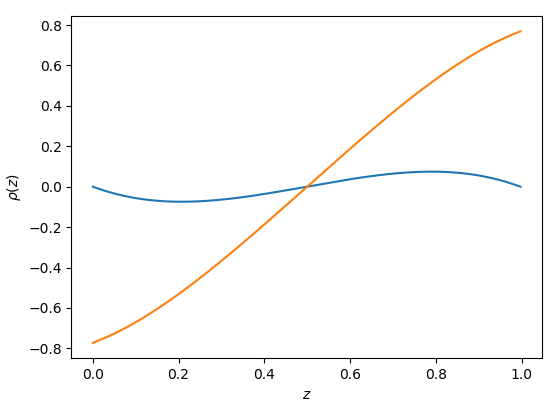
\includegraphics[width=0.9\textwidth]{figures/renormalization_comparison_rho.png}
	    	    \end{figure}
	    \end{column}
	    \begin{column}{0.5\textwidth}
	    	   The induced charge density $\rho$ resulting from the two different renormalization techniques with Dirichlet boundary conditions. In orange the one calculated through the mode sum formula and in blue the one calculated through Hadamard point-splitting. This is a particular case for $m = 0$, $\lambda = 5$,  $a=1$.
	    \end{column}
	\end{columns}
	    \end{frame}

\begin{frame}{The induced fields}
	\begin{columns}
		\uncover<1->{
		        \begin{column}{0.5\textwidth}
		    	    The induced electric field:
		    	    \begin{align}
		    	    \tilde{E}(z) = \int_{0}^{z} \rho(z')dz' 
		    	    \end{align}
		        \begin{figure}[h]
		        	\centering
		        	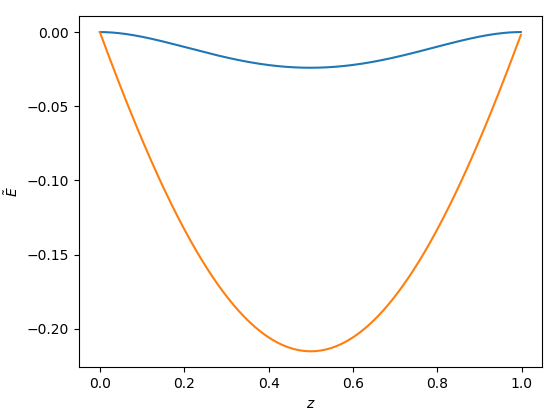
\includegraphics[width=0.8\textwidth]{figures/renormalization_comparison_induced_E.png}
		        \end{figure}
		        \end{column}
		}
		
		\uncover<2->{
		    
	    \begin{column}{0.5\textwidth}
		    	    The induced electric potential
		    	    \begin{align}
	\tilde{A_0}(z) = -\int_{0}^{z} \tilde{E}(z') dz'
		    	    \end{align}
		        \begin{figure}[h]
		        	\centering
		        	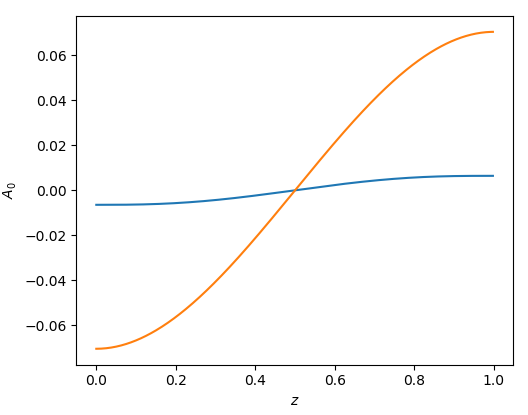
\includegraphics[width=0.8\textwidth]{figures/renormalization_comparison_induced_A0.png}
		        \end{figure}
		        \end{column}
		}
	\end{columns}
\end{frame}

\begin{frame}{Closing the loop}

\begin{align}
			\left(
				\left[ 
			\omega^{\left( \kappa \right) }_n 
	+ \lambda \left( z - \frac{1}{2} \right) 
- \epsilon \tilde{A}^{\left(\kappa  \right) }_0(z)  \right]^2 
	+ \frac{d^2}{dz^2} + a^2m^2  \right)
	\phi^{\left( \kappa + 1 \right) }_n &= 0 \\
	\tilde{A_0}^{(\kappa)}(z) = -\int_{0}^{z} \int_{0}^{z'} \rho^{(\kappa)}(z'')dz''   dz'
,
\end{align}
\end{frame}

\begin{frame}{Closing the loop}
	
\begin{tikzpicture}[
    box/.style = {draw, rectangle, minimum width=2cm, minimum height=1cm},
    arrow/.style = {->, thin, >=Stealth},
    curved arrow/.style = {->, thick, >=Stealth, bend left}
]
\begin{centering}
	

% Nodes
\node[box] (A0) {$A_0^{(\kappa=0)}$};
\node[box, right=1cm of A0] (phi) {$\phi$};
\node[box, above right=1cm and 2cm of phi] (rho) {$\rho$};
\node[box, below right=1cm and 2cm of phi] (tildeA0) {$A^{\phi}_0^{\left( \kappa \right) }$};

% Curved arrows for the loop
\draw[arrow] (A0) -- (phi);
\draw[curved arrow, red] (phi) to[out=45, in=135] (rho);
\draw[curved arrow, red] (rho) to[out=45, in=135] (tildeA0);
\draw[curved arrow, red] (tildeA0) to[out=45, in=135] (phi);

% Center arrow with text
\node[right=0.9cm of phi] (kappa) {$\kappa \to \infty$};
 \draw[arrow, blue] (6.5, -0.25) arc [start angle=345, end angle=15, radius=1cm];


\end{centering}\end{tikzpicture}

\end{frame}

% \begin{frame}[fragile]{}
% \framesubtitle{Selecting the Theme}
% To start working with \texttt{beamer\_statale}, start a \LaTeX\ document with the preamble:
% \testcolor{\useBlockTitleColor}, \testcolor{\useBlockMainColor} (see section \ref{Themes})
% \begin{themedTitleBlock}{Block title}
%     It can be useful to treat some content differently by putting it into a block. This can be done by using blocks!
% \end{themedTitleBlock}
% \end{frame}
% 
% %=======================================================================
% 
% \begin{frame}[fragile]{Title page}
% To set a typical title page, you call some commands in the preamble:
% \begin{block}{The Commands for the Title Page}
% \begin{verbatim}
% \title{A basic presentation template}
% \subtitle{for the Universität Regensburg}
% 
% \Author{Antoine Gansel}
% \AuthorInstitute{Lehrstuhl für Datensicherheit und Kryptographie}
% \Collaborators{{Julie Cailler\inst{2}}} 
% \Supervisors{Jane Doe\inst{1} \and {John Doe\inst{2}}}
% \institute{{\inst{1}UR - Lehrstuhl für Datensicherheit und [...]}}
% \end{verbatim}
% \end{block}
% 
% You can comment/delete any of \verb|\Collaborators{...}|, \verb|\Supervisors{...}| and \verb|\institute{...}| without issue.
% 
% \end{frame}
% 
% %=======================================================================
% 
% \begin{frame}[fragile]{Writing a Simple Slide}
% \framesubtitle{It's really easy!}
% \begin{itemize}[<+->]
%     \item A typical slide has bulleted lists
%     \item These can be uncovered in sequence
% \end{itemize}
% \begin{block}{Code for a Page with an Itemised List}<+->
% \begin{verbatim}
% \begin{frame}{Writing a Simple Slide}
%     \framesubtitle{It's really easy!}
%         \begin{itemize}[<+->]
%             \item A typical slide has bulleted lists
%         \item These can be uncovered in sequence
% \end{itemize}\end{frame}
% \end{verbatim}
% \end{block}
% \end{frame}
% 
% %=======================================================================
% 
% \begin{frame}{Uncovering in sequence}
%     \centering \textbf{You can do that with pretty much anything !} \\
%     \uncover<2->{Pictures from \url{https://www.shutterstock.com/en/g/lantoine}}
%     \begin{columns}  % adding [onlytextwidth] the left margins will be set correctly
%         \begin{column}{0.50\textwidth}
%             \begin{center}
% 		%\uncover<2->{
\includegraphics[height=0.6\textheight]{Config/Souris.png}}
%             \end{center}
%         \end{column}
%         \begin{column}{0.50\textwidth}
%             \begin{center}
%                 %\uncover<3->{
\includegraphics[height=0.6\textheight]{Config/Poulpe.png}}
%             \end{center}
%         \end{column}
%     \end{columns}
% \end{frame}
